
{\actuality} 
В настоящее время задача улучшения производительности вычислительных машин приобретает всё большее значение. В 2021 году две трети населения планеты ежедневно использовали мобильные вычислительные устройства, а их количество стало больше 4 миллиардов. Уменьшение времени работы на конкретных задачах или увеличение соотношения производительность/энергопотребление приносит большой выигрыш в масштабе количества устройств.

Повышения производительности приложений можно добиться двумя способами: улучшением аппаратного и программного обеспечения. Под программным обеспечением понимается не только качество написанного кода и выбранных алгоритмов, но и процесс трансляции высокоуровневого языка в бинарное представление вместе с процессом запуска бинарного файла. Для повышения производительности в трансляцию добавляются оптимизирующие стадии, такие как оптимизации компилятора, линкера и бинарные оптимизации. Последние могут быть использованы в случаях, когда в наличии есть только исполняемый бинарный файл приложения, что применимо при отсутствии исходного кода (рисунок \cref{fig:Compile}).

Для повышения качества оптимизаций на вход трансляторам может поступать дополнительная информация: профиль исполнения, вероятные входные данные, дополнительная данные о микроархитектуре целевого процессора и др.

\begin{figure}[ht]
    \centerfloat{
        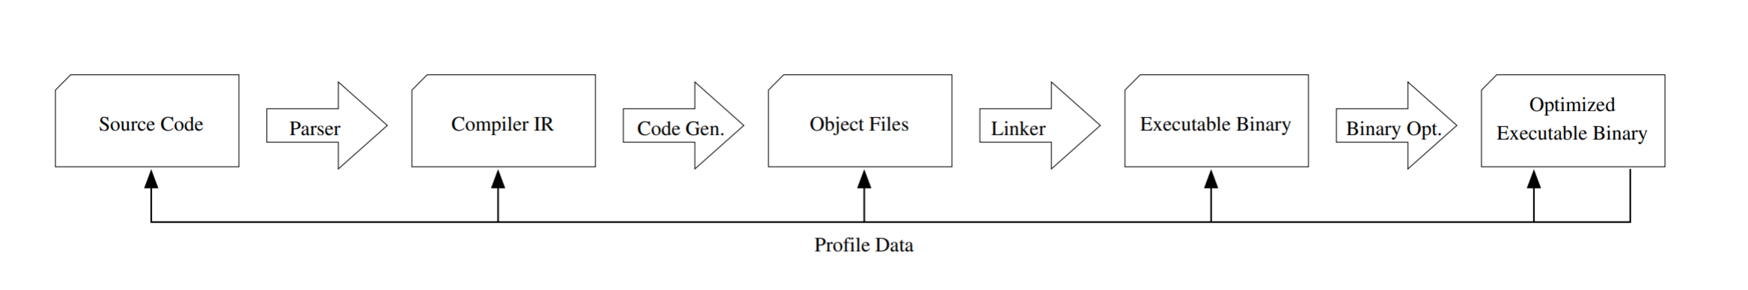
\includegraphics[width=1.0\linewidth]{translation}
    }
    \caption{Процесс трансляции исходного кода в оптимизированный бинарный файл}\label{fig:Compile}
\end{figure}

Оптимизация приложений является важнейшей частью процесса создания современного программного обеспечения, так как позволяет в разы повысить производительность и энергоэффективность вычислений. Оптимизации на основе профильной информации приложения позволяют получить большой прирост в указанных выше параметрах. Для получения профиля нужно использовать специально собранную версию приложения либо обеспечивать аппаратную поддержку сбора необходимых характеристик.

Для архитектуры x86 существует специальная аппаратная поддержка, позволяющая собирать профильную информацию во время исполнения приложения - LBR (Last Branch Record). Для ARM архитектуры аналог данной технологии существует, но не поддерживается всеми процессорами, что создаёт проблемы для оптимизаций приложений с учётом профиля исполнения. Произвести статическую инструментацию приложения не всегда является возможным, например, в случае отсутствия исходного кода или информации о символах и релокационных данных в бинарном файле. Поэтому \textbf{актуальной} задачей является разработка метода получения профильной информации для ARM архитектуры и дополнительных бинарных оптимизаций.

{\aim} данной работы является изучение и оптимизация существующих инструментов статической бинарной трансляции под RISC архитектуры. Основной целевой платформой является одна из наиболее распространенных на данный момент RISC архитектур -- ARM. Основным классом оптимизаций являются оптимизации, использующие профильную информацию исполнения приложения.

Для~достижения поставленной цели необходимо было решить следующие {\tasks}:
\begin{enumerate}[beginpenalty=10000] % https://tex.stackexchange.com/a/476052/104425
  \item Исследовать существующие статические бинарные трансляторы под RISC архитектуры.
  \item Разработать универсальный метод получения профильной информации под RISC архитектуры.
  \item Разработать ПО для получения профильной информации приложения по трассе его исполнения.
  \item Разработать методы улучшения статического бинарного транслятора.
  \item Реализовать наиболее перспективные методы улучшения бинарного оптимизатора.
  \item Разработать новые оптимизации на основе внедренных методов и улучшений.
  \item Протестировать разработанные методы на реальных приложениях под RISC архитектуру.
\end{enumerate}

Тема и содержание диссертационной работы соответствует паспорту научной специальности 05.13.11 – Математическое и программное обеспечение вычислительных машин, комплексов и компьютерных сетей, в частности, пунктам:

п. 1 – Модели, методы и алгоритмы проектирования и анализа программ и программных систем, их эквивалентных преобразований, верификации и тестирования.

п. 3 – Модели, методы, алгоритмы, языки и программные инструменты для организации взаимодействия программ и программных систем.

{\novelty}
\begin{enumerate}[beginpenalty=10000] % https://tex.stackexchange.com/a/476052/104425
  \item В диссертационной работе был реализован новый алгоритм получения профильной информации формата BOLT на основе трасс исполнения приложения. В диссертации показано, что для определенных классов устройств это единственный способ получения полноценного профиля приложения.
  \item Была реализована полноценная поддержка бинарного оптимизатора BOLT для ARM архитектуры, необходимая для проведения тестовых замеров на целевых приложениях, в то время как исходная версия BOLT не поддерживает оптимизацию нужных приложений.
  \item Был разработан специальный формат, описывающий преобразования исполняемого файла в оптимизированный.
  \item Был разработан статический анализатор, верифицирующий оптимизированный исполняемый файл на основе оригинального файла и файла преобразования.
  \item Был создан алгоритм мультипрофильного анализа, выделяющий профили приложения на основе трасс исполнения. На его основе реализована оптимизация копирования кода.

\end{enumerate}

{\influence} данной работы заключается в использовании разработанных методов и алгоритмов в бинарном оптимизаторе BOLT и его инфраструктуре и успешном \textbf{внедрении} компанией ООО <<Техкомпания Хуавэй>> для оптимизации приложений. Реализованные оптимизации, верификации и методы получения профильной информации позволили получить прирост производительности на целевых приложениях компании.

Результаты данной работы также \textbf{внедрены} в кафедральный курс «Современные методы разработки компиляторов» кафедры микропроцессорных технологий в интеллектуальных системах управления МФТИ.

Теоретическая значимость диссертационной работы заключается в разработке новых методов использования трасс исполнения приложения, как для получения профильной информации, так и для использования в анализе и оптимизациях.

{\defpositions}
\begin{enumerate}[beginpenalty=10000] % https://tex.stackexchange.com/a/476052/104425
  \item Метод получения профильной информации для бинарного оптимизатора BOLT из трасс исполнения приложений.
  \item Алгоритм оптимизации длинных переходов при работе бинарного оптимизатора BOLT.
  \item Алгоритм верификации оптимизированных бинарным оптимизатором BOLT файлов.
  \item Алгоритм мультипрофильного анализа трасс исполнения приложений.
  \item Алгоритм дублирования кода на основе мультипрофильного анализа трасс исполнения приложений.
\end{enumerate}

{\reliability}
Обоснованность и достоверность результатов и выводов диссертации подтверждается подробным описанием проведенных экспериментов и полученных данных.

{\probation}
Результаты диссертационной работы докладывались на следующих научно-технических конференциях:
\begin{enumerate}[beginpenalty=10000] % https://tex.stackexchange.com/a/476052/104425
  \item 63-й всероссийской научной конференции московского физико–технического института (государственного университета, Москва, ноябрь 2020 г.
  \item Международном конгрессе <<Современные проблемы компьютерных и информационных наук>>, Москва, ноябрь 2021 г.
  \item 64-й всероссийской научной конференции московского физико–технического института (государственного университета, Москва, ноябрь 2021 г.
\end{enumerate}

{\contribution} Основные результаты диссертационного исследования получены лично автором. Постановка задач и анализ полученных результатов осуществлялся непосредственно автором. В совместных работах вклад автора в результаты исследования являлся определяющим. Автор лично реализовывал и интегрировал разработанные решения в бинарный оптимизатор BOLT.

\ifnumequal{\value{bibliosel}}{0}
{%%% Встроенная реализация с загрузкой файла через движок bibtex8. (При желании, внутри можно использовать обычные ссылки, наподобие `\cite{vakbib1,vakbib2}`).
    {\publications} Основные результаты по теме диссертации изложены
    в~XX~печатных изданиях,
    X из которых изданы в журналах, рекомендованных ВАК,
    X "--- в тезисах докладов.
}%
{%%% Реализация пакетом biblatex через движок biber
    \begin{refsection}[bl-author, bl-registered]
        % Это refsection=1.
        % Процитированные здесь работы:
        %  * подсчитываются, для автоматического составления фразы "Основные результаты ..."
        %  * попадают в авторскую библиографию, при usefootcite==0 и стиле `\insertbiblioauthor` или `\insertbiblioauthorgrouped`
        %  * нумеруются там в зависимости от порядка команд `\printbibliography` в этом разделе.
        %  * при использовании `\insertbiblioauthorgrouped`, порядок команд `\printbibliography` в нём должен быть тем же (см. biblio/biblatex.tex)
        %
        % Невидимый библиографический список для подсчёта количества публикаций:
        \printbibliography[heading=nobibheading, section=1, env=countauthorvak,          keyword=biblioauthorvak]%
        \printbibliography[heading=nobibheading, section=1, env=countauthorwos,          keyword=biblioauthorwos]%
        \printbibliography[heading=nobibheading, section=1, env=countauthorscopus,       keyword=biblioauthorscopus]%
        \printbibliography[heading=nobibheading, section=1, env=countauthorconf,         keyword=biblioauthorconf]%
        \printbibliography[heading=nobibheading, section=1, env=countauthorother,        keyword=biblioauthorother]%
        \printbibliography[heading=nobibheading, section=1, env=countregistered,         keyword=biblioregistered]%
        \printbibliography[heading=nobibheading, section=1, env=countauthorpatent,       keyword=biblioauthorpatent]%
        \printbibliography[heading=nobibheading, section=1, env=countauthorprogram,      keyword=biblioauthorprogram]%
        \printbibliography[heading=nobibheading, section=1, env=countauthor,             keyword=biblioauthor]%
        \printbibliography[heading=nobibheading, section=1, env=countauthorvakscopuswos, filter=vakscopuswos]%
        \printbibliography[heading=nobibheading, section=1, env=countauthorscopuswos,    filter=scopuswos]%
        %
        \nocite{*}%
        %
        {\publications} Основные результаты по теме диссертации изложены в~\arabic{citeauthor}~печатных изданиях,
        \arabic{citeauthorvak} из которых изданы в журналах, рекомендованных ВАК\sloppy%
        \ifnum \value{citeauthorscopuswos}>0%
            , \arabic{citeauthorscopuswos} "--- в~периодических научных журналах, индексируемых Web of~Science и Scopus\sloppy%
        \fi%
        \ifnum \value{citeauthorconf}>0%
            , \arabic{citeauthorconf} "--- в~тезисах докладов.
        \else%
            .
        \fi%
        \ifnum \value{citeregistered}=1%
            \ifnum \value{citeauthorpatent}=1%
                Зарегистрирован \arabic{citeauthorpatent} патент.
            \fi%
            \ifnum \value{citeauthorprogram}=1%
                Зарегистрирована \arabic{citeauthorprogram} программа для ЭВМ.
            \fi%
        \fi%
        \ifnum \value{citeregistered}>1%
            Зарегистрированы\ %
            \ifnum \value{citeauthorpatent}>0%
            \formbytotal{citeauthorpatent}{патент}{}{а}{}\sloppy%
            \ifnum \value{citeauthorprogram}=0 . \else \ и~\fi%
            \fi%
            \ifnum \value{citeauthorprogram}>0%
            \formbytotal{citeauthorprogram}{программ}{а}{ы}{} для ЭВМ.
            \fi%
        \fi%
        % К публикациям, в которых излагаются основные научные результаты диссертации на соискание учёной
        % степени, в рецензируемых изданиях приравниваются патенты на изобретения, патенты (свидетельства) на
        % полезную модель, патенты на промышленный образец, патенты на селекционные достижения, свидетельства
        % на программу для электронных вычислительных машин, базу данных, топологию интегральных микросхем,
        % зарегистрированные в установленном порядке.(в ред. Постановления Правительства РФ от 21.04.2016 N 335)
    \end{refsection}%
    \begin{refsection}[bl-author, bl-registered]
        % Это refsection=2.
        % Процитированные здесь работы:
        %  * попадают в авторскую библиографию, при usefootcite==0 и стиле `\insertbiblioauthorimportant`.
        %  * ни на что не влияют в противном случае
        \nocite{vakbib1}%vak
        \nocite{vakbib2}%vak
        \nocite{confbib1}%conf
        \nocite{confbib2}%conf
        \nocite{confbib3}%conf
    \end{refsection}%
        %
        % Всё, что вне этих двух refsection, это refsection=0,
        %  * для диссертации - это нормальные ссылки, попадающие в обычную библиографию
        %  * для автореферата:
        %     * при usefootcite==0, ссылка корректно сработает только для источника из `external.bib`. Для своих работ --- напечатает "[0]" (и даже Warning не вылезет).
        %     * при usefootcite==1, ссылка сработает нормально. В авторской библиографии будут только процитированные в refsection=0 работы.
}